\documentclass[tikz, border=5pt]{standalone}
\usepackage[dvipsnames]{xcolor}
\usepackage{tikz}
\usetikzlibrary{arrows.meta,calc,fit,positioning,backgrounds}

\tikzset{
    portbox/.style={
        rectangle,
        draw=gray!50!black,
        fill=gray!12,
        rounded corners=2pt,
        minimum width=15mm,
        minimum height=10mm,
        inner sep=2pt,
        align=center
    },
    layerbox/.style={
        rectangle,
        draw=gray!45,
        fill=gray!6,
        rounded corners=2pt,
        line width=0.5pt
    },
    arrow/.style={
        ->,
        thick,
        >=Latex
    },
    biarrow/.style={
        <->,
        thick,
        >=Latex
    },
    activemodelbox/.style={
        rectangle,
        draw=green!60!black,
        fill=green!18,
        rounded corners=2pt,
        minimum width=20mm,
        minimum height=10mm,
        inner sep=4pt,
        align=center,
        very thick
    },
    inactivemodelbox/.style={
        rectangle,
        draw=green!55,
        fill=green!8,
        rounded corners=2pt,
        minimum width=20mm,
        minimum height=10mm,
        inner sep=4pt,
        align=center,
    },
    helperbox/.style={
        rectangle,
        draw=orange!50!black,
        fill=orange!12,
        rounded corners=2pt,
        minimum width=20mm,
        minimum height=10mm,
        inner sep=4pt,
        align=center
    },
    selectarrow/.style={
    ->,
    dashed,
    line width=0.8pt,
    draw=orange!70!black,
    >=Latex
    },
    supportarrow/.style={
    ->,
    line width=0.8pt,
    draw=orange!65!black,
    >=Latex
}
}

\begin{document}
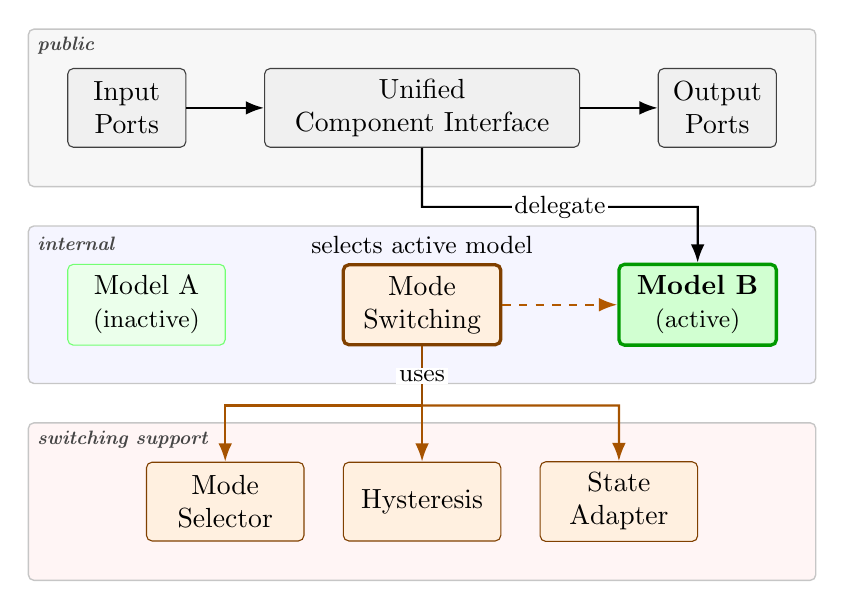
\begin{tikzpicture}
    % Public interface layer
    \begin{scope}[yshift=4.5cm]
        \node[layerbox, minimum width=10cm, minimum height=2cm] (publiclayer) at (4.5,0) {};
        \node[anchor=south west, font=\scriptsize\bfseries\itshape, text=gray!55!black]
            at ($(publiclayer.north west)+(0,-0.45)$) {public};

        \node[portbox, align=center] (In) at (0.75,0) {Input\\Ports};
        \node[portbox, align=center] (Out) at (8.25,0) {Output\\Ports};
        \node[portbox, align=center, minimum width=40mm] (interface) at (4.5, 0) {Unified\\Component Interface};

        \draw[arrow] (In) -- (interface);
        \draw[arrow] (interface) -- (Out);
    \end{scope}

    % Internal layer
    \begin{scope}
        \node[layerbox, fill=blue!4, minimum width=10cm, minimum height=2cm] (internallayer) at (4.5,2) {};
        \node[anchor=south west, font=\scriptsize\bfseries\itshape, text=gray!55!black]
            at ($(internallayer.north west)+(0,-0.45)$) {internal};
        \node[inactivemodelbox, align=center] (modelA)   at (1, 2)  {Model A\\{\small(inactive)}};
        \node[activemodelbox, align=center]   (modelB)   at (8, 2)  {\textbf{Model B}\\{\small(active)}};
        \node[helperbox, align=center, very thick]        (switching) at (4.5,2) {Mode\\Switching};
        \node[above, font=\small, align=center] at (switching.north){selects active model};

        % --- Control relationships: switcher activates/deactivates models ---
        \draw[selectarrow] (switching.east) -- (modelB.west);
    \end{scope}

    % Switching support layer
    \begin{scope}[yshift=-0.5cm]
        \node[layerbox, fill=red!4, minimum width=10cm, minimum height=2cm] (switchingsupport) at (4.5,0) {};
        \node[anchor=south west, font=\scriptsize\bfseries\itshape, text=gray!55!black]
            at ($(switchingsupport.north west)+(0,-0.45)$) {switching support};
        \node[helperbox, align=center] (selector)   at (2,   0) {Mode\\Selector};
        \node[helperbox, align=center] (hysteresis) at (4.5, 0) {Hysteresis};
        \node[helperbox, align=center] (adapter)    at (7,   0) {State\\Adapter};
    \end{scope}

    % --- Data path: interface delegates to whichever model is active ---
    \draw[arrow] (interface.south) --++(0, -0.75)
                                   --++(3.5, 0) node[midway, font=\small, fill=white, inner sep=1pt] {delegate} 
                                   -- (modelB.north);
    \coordinate (supportJunction) at ($(switching.south)+(0,-0.75)$);

    \draw[thick, draw=orange!60!black]
    (switching.south) -- node[midway, font=\small, fill=white, inner sep=1pt] {uses} (supportJunction);

    \draw[supportarrow]
    (supportJunction) -- (hysteresis.north);

    \draw[supportarrow]
    (supportJunction) --++ (2.5, 0) -- (adapter.north);

    \draw[supportarrow]
    (supportJunction) --++ (-2.5, 0) -- (selector.north);

    % Helpers
    \useasboundingbox (-0.5, -1.5) rectangle (9.5, 5.5);
    % \draw[help lines, step=0.5, draw=gray!50, very thin] (-0.5,-1.5) grid (9.5, 5.5);


\end{tikzpicture}
\end{document}
